\documentclass{scrreprt}
\usepackage[bookmarks=true]{hyperref}
\usepackage{tabto}
\usepackage{epsfig}
\usepackage{epstopdf}
\hypersetup{%
    pdftitle={Functional Requirement Specification},    % title
    colorlinks=true,       % false: boxed links; true: colored links
    linkcolor=blue,       % color of internal links
    citecolor=black,       % color of links to bibliography
    filecolor=black,        % color of file links
    urlcolor=purple,        % color of external links
    linktoc=page            % only page is linked
}
\title
{%
\author
{
Khathutshelo Matidza 11072157\\
\and
Renaldo van Dyk 12204359\\
\and
Andreas du Preez 12207871\\
\and
Sean Hill 12221458\\
\and
Kgomotso Sito 12243273\\
\and
Hlavutelo Maluleke 12318109\\
\and
Sboniso Masilela 10416260\\
\and
Semaka Malapane 13081129\\
}	
\centering

\includegraphics[scale=.9]{graphics/universityLogo.jpg}\\
\vspace{2cm}
\huge{COS301: Mini Project-Phase 1\\Functional Requirements}\\
\vspace{2cm}
Buzz System\\
\vspace{2cm}
GitHub\\
\LARGE\texttt{https://github.com/RenaldoV/COS301\_Group5\_a}
\vfill
\vspace{1cm}
\rule{15cm}{2pt}
}
\date
{}
\usepackage{hyperref}
\begin{document}
\maketitle
\tableofcontents
\chapter{Introduction}
The Computer Science Education Didactic and Applications Research (CSEDAR) team of the Computer Science Department of the University of Pretoria have registered a research project called “The use of Online Discussions in Teaching (TODT)”. The aims of this research is to find ways to enhance teaching and improve the learning of students through the use of online discussions. The formation of collaborative communities within student groups has become essential to enhance education. The existence of a forum in which students can express their views and explore what they are learning results in creating a collaborative community in which students can excel. We are faced with the problem of engaging an extremely large number of first year students. Engaging first year students is a difficult and well-recognised problem, since students tend to feel part of an anonymous mass. As part of the TODT project as a whole, the aim of this COS 301 project is to create an online space where students, teaching assistants and lecturers can engage in activities related to learning the content of our module while applying game concepts to motivate students to increase the quality of their participation and consequently experience deeper learning of the course content.
\\
\chapter{Use Case Prioritization: AdminManagement}

\section{Critical}
2.1 createAccount\\
2.2 deleteAccount\\
\section{Important}

\section{Nice-To-Have}
2.3 customizeInterface\\
2.4 summarizeThreads\\

\chapter{Use Case/Services Contracts: AdminManagement}
\NumTabs{18}

\section{Pre-Conditions}								%PRE CONDITIONS
2.1\tab{a) User must be registered for COS301}\\
2.2\tab{a) User must have completed COS301}\\
2.2\tab{b) User must have graduated/no longer a personel/student at the university}\\
2.3\tab{a) User status level should be staff}\\
2.4\tab{a) User status level should be staff}\\

\section{Post-Conditions}								%POST CONDITIONS	
2.1\tab{a) User details should be visible on Buzz profiles}\\
2.1\tab{b) User should be able to CRUD depending on status level}\\
2.2\tab{a) User should no longer exist nor should any of the previous activities}\\
2.3\tab{a) Threads should be hidden/closed and moved around}\\
2.4\tab{a) Threads should be summarized accordingly}\\

\section{Request and Results Data Structures} 
\NumTabs{18}
\chapter{Required Functionality: AdminManagement}
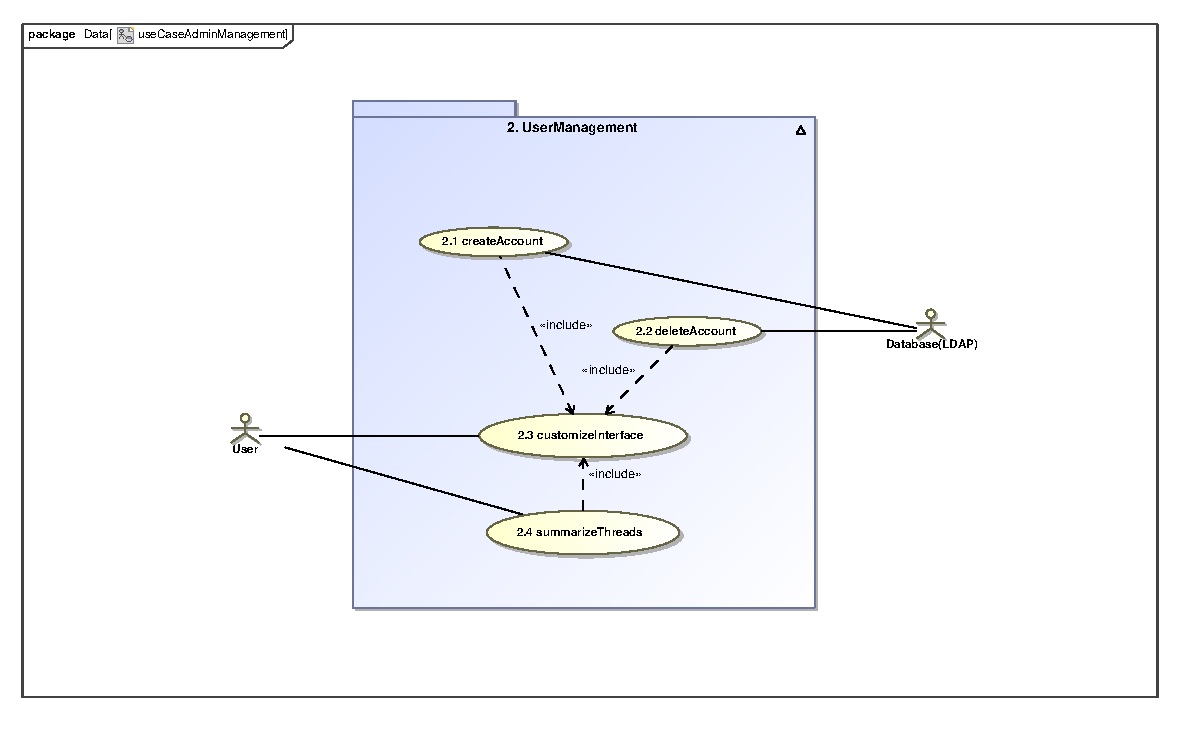
\includegraphics[scale=.9]{graphics/useCaseAdminManagement.eps}\\

\chapter{Process Specifications: AdminManagement}
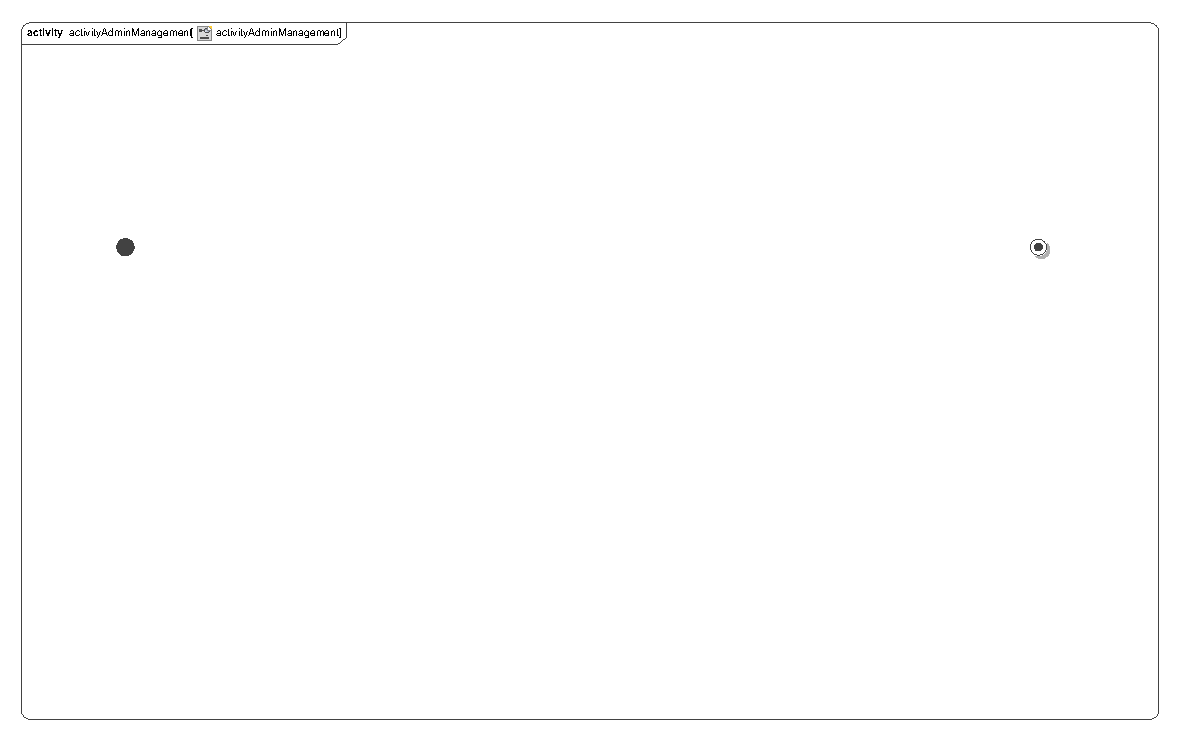
\includegraphics[scale=.9]{graphics/activityAdminManagement.eps}\\

\chapter{Domain Model}
\NumTabs{18}

\chapter{High Level Overview}
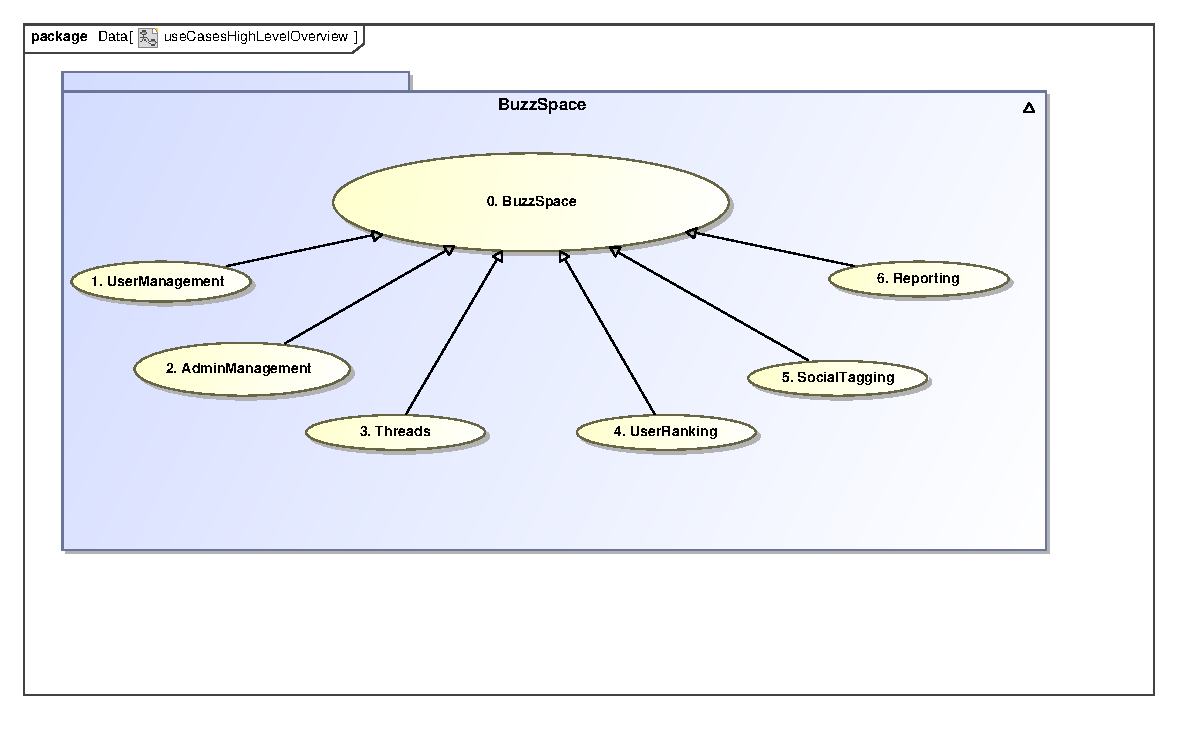
\includegraphics[scale=.9]{graphics/useCasesHighLevelOverview.eps}\\

\end{document}